% Options for packages loaded elsewhere
\PassOptionsToPackage{unicode}{hyperref}
\PassOptionsToPackage{hyphens}{url}
\PassOptionsToPackage{dvipsnames,svgnames,x11names}{xcolor}
%
\documentclass[
  12pt,
]{article}
\usepackage{amsmath,amssymb}
\usepackage{lmodern}
\usepackage{iftex}
\ifPDFTeX
  \usepackage[T1]{fontenc}
  \usepackage[utf8]{inputenc}
  \usepackage{textcomp} % provide euro and other symbols
\else % if luatex or xetex
  \usepackage{unicode-math}
  \defaultfontfeatures{Scale=MatchLowercase}
  \defaultfontfeatures[\rmfamily]{Ligatures=TeX,Scale=1}
\fi
% Use upquote if available, for straight quotes in verbatim environments
\IfFileExists{upquote.sty}{\usepackage{upquote}}{}
\IfFileExists{microtype.sty}{% use microtype if available
  \usepackage[]{microtype}
  \UseMicrotypeSet[protrusion]{basicmath} % disable protrusion for tt fonts
}{}
\makeatletter
\@ifundefined{KOMAClassName}{% if non-KOMA class
  \IfFileExists{parskip.sty}{%
    \usepackage{parskip}
  }{% else
    \setlength{\parindent}{0pt}
    \setlength{\parskip}{6pt plus 2pt minus 1pt}}
}{% if KOMA class
  \KOMAoptions{parskip=half}}
\makeatother
\usepackage{xcolor}
\usepackage[margin=1in]{geometry}
\usepackage{longtable,booktabs,array}
\usepackage{calc} % for calculating minipage widths
% Correct order of tables after \paragraph or \subparagraph
\usepackage{etoolbox}
\makeatletter
\patchcmd\longtable{\par}{\if@noskipsec\mbox{}\fi\par}{}{}
\makeatother
% Allow footnotes in longtable head/foot
\IfFileExists{footnotehyper.sty}{\usepackage{footnotehyper}}{\usepackage{footnote}}
\makesavenoteenv{longtable}
\usepackage{graphicx}
\makeatletter
\def\maxwidth{\ifdim\Gin@nat@width>\linewidth\linewidth\else\Gin@nat@width\fi}
\def\maxheight{\ifdim\Gin@nat@height>\textheight\textheight\else\Gin@nat@height\fi}
\makeatother
% Scale images if necessary, so that they will not overflow the page
% margins by default, and it is still possible to overwrite the defaults
% using explicit options in \includegraphics[width, height, ...]{}
\setkeys{Gin}{width=\maxwidth,height=\maxheight,keepaspectratio}
% Set default figure placement to htbp
\makeatletter
\def\fps@figure{htbp}
\makeatother
\setlength{\emergencystretch}{3em} % prevent overfull lines
\providecommand{\tightlist}{%
  \setlength{\itemsep}{0pt}\setlength{\parskip}{0pt}}
\setcounter{secnumdepth}{5}
\newlength{\cslhangindent}
\setlength{\cslhangindent}{1.5em}
\newlength{\csllabelwidth}
\setlength{\csllabelwidth}{3em}
\newlength{\cslentryspacingunit} % times entry-spacing
\setlength{\cslentryspacingunit}{\parskip}
\newenvironment{CSLReferences}[2] % #1 hanging-ident, #2 entry spacing
 {% don't indent paragraphs
  \setlength{\parindent}{0pt}
  % turn on hanging indent if param 1 is 1
  \ifodd #1
  \let\oldpar\par
  \def\par{\hangindent=\cslhangindent\oldpar}
  \fi
  % set entry spacing
  \setlength{\parskip}{#2\cslentryspacingunit}
 }%
 {}
\usepackage{calc}
\newcommand{\CSLBlock}[1]{#1\hfill\break}
\newcommand{\CSLLeftMargin}[1]{\parbox[t]{\csllabelwidth}{#1}}
\newcommand{\CSLRightInline}[1]{\parbox[t]{\linewidth - \csllabelwidth}{#1}\break}
\newcommand{\CSLIndent}[1]{\hspace{\cslhangindent}#1}
\usepackage{setspace} \setstretch{1.15} \usepackage{float} \floatplacement{figure}{t}
\ifLuaTeX
  \usepackage{selnolig}  % disable illegal ligatures
\fi
\IfFileExists{bookmark.sty}{\usepackage{bookmark}}{\usepackage{hyperref}}
\IfFileExists{xurl.sty}{\usepackage{xurl}}{} % add URL line breaks if available
\urlstyle{same} % disable monospaced font for URLs
\hypersetup{
  colorlinks=true,
  linkcolor={cyan},
  filecolor={Maroon},
  citecolor={Blue},
  urlcolor={cyan},
  pdfcreator={LaTeX via pandoc}}

\title{~\Large Increased sexual dimorphism evolves in a fossil
stickleback following ecological release from fish piscivores}
\author{\large Allison Ozark\(^{1,*}\), Matthew Stuart\(^{2,3,*}\),
Raheyma Siddiqui\(^1\), Akhil Ghosh\(^2\)\\
\large Samantha Swank\(^1\), Michael A. Bell\(^4\), Gregory J.
Matthews\(^{2,3}\), and Yoel E. Stuart\(^{1,+}\)\\
\vspace{-1.1mm}\\
\large \(^1\) Department of Biology, Loyola University Chicago, Chicago,
IL, USA \vspace{-1.1mm}\\
\large \(^2\) Department of Mathematics and Statistics, Loyola
University Chicago, Chicago, IL, USA \vspace{-1.1mm}\\
\large \(^3\) Center for Data Science and Consulting, Loyola University
Chicago, Chicago, IL, USA \vspace{-1.1mm}\\
\large \(^4\) University of California Museum of Paleontology, Berkeley,
CA, USA \vspace{-1.1mm}\\
\large \(^*\) Equal contribution \vspace{-1.1mm}\\
\large \(^+\) Corresponding:
\href{mailto:ystuart@luc.edu}{\nolinkurl{ystuart@luc.edu}}
\vspace{-1.1mm}}
\date{}

\begin{document}
\maketitle
\begin{abstract}
Everyone loves the stickle \vspace{2mm}\\
\emph{Keywords}: Stickle
\end{abstract}

\newcommand{\iid}{\overset{iid}{\sim}}

\newpage

\hypertarget{sec:intro}{%
\section{Introduction}\label{sec:intro}}

Ecological release theory suggests that a prey population's niche should
expand when predation is relaxed or removed, as prey take advantage of
new enemy free space (reviewed in Herrmann, Stroud, and Losos
(\protect\hyperlink{ref-Herrmann2021}{2021})). Niche expansion could
manifest through a combination of increasing within- and
between-individual niche widths (Bolnick et al.
(\protect\hyperlink{ref-Bolnick2010}{2010}); Herrmann, Stroud, and Losos
(\protect\hyperlink{ref-Herrmann2021}{2021})), including divergence
between the sexes (Bolnick and Doebeli
(\protect\hyperlink{ref-Bolnick2003}{2003}); Cooper, Gilman, and
Boughman (\protect\hyperlink{ref-Cooper2011}{2011})). Theory and
empirical data suggest that a population presented with ecological
opportunity following ecological release might experience disruptive
selection on males and females stemming from intraspecific competition
over newly accessible resources, resulting in intersexual divergence in
habitat use (W. (\protect\hyperlink{ref-Schoener1968}{1968}); Shine
(\protect\hyperlink{ref-Shine1989}{1989}); Bolnick and Doebeli
(\protect\hyperlink{ref-Bolnick2003}{2003}); Butler, Sawyer, and Losos
(\protect\hyperlink{ref-Butler2007}{2007}); Bolnick and Lau
(\protect\hyperlink{ref-Bolnick2008}{2008}); Cooper, Gilman, and
Boughman (\protect\hyperlink{ref-Cooper2011}{2011}); but see Stuart et
al. (\protect\hyperlink{ref-Stuart2021}{2021}); Blain
(\protect\hyperlink{ref-Blain2022}{2022})). Accordingly, sexes should
also diverge in morphological traits associated with habitat use; such
ecologically-driven ``character displacement between the sexes'' is
therefore one explanation for phenotypic sexual dimorphism (S. P. De
Lisle and Rowe (\protect\hyperlink{ref-deLisleRowe2015}{2015}); S. Paiva
De Lisle S. P. and Rowe (\protect\hyperlink{ref-deLisleNco2018}{2018})).

We tested this link between release from predators and the evolution of
sexual dimorphism in a well-preserved, finely-resolved,
\textasciitilde16,000 year-long sequence of the fossil stickleback fish
(Gasterosteus doryssus). The fossil lineage appeared in the depositional
environment as a fully armored form, with complete pelvic girdles, two
pelvic spines, and three dorsal spines, on average (Michael A. Bell,
Travis, and Blouw (\protect\hyperlink{ref-Bell2006}{2006}); Stuart,
Travis, and Bell (\protect\hyperlink{ref-Stuart2020}{2020})). However,
this habitat appears to have been missing fish piscivores (e.g., trout
and other salmonids known to prey on modern stickleback; M. A. Bell
(\protect\hyperlink{ref-Bell2009}{2009})), relaxing putative selection
for armor (T. E. Reimchen (\protect\hyperlink{ref-Reimchen1980}{1980}),
T. E. Reimchen (\protect\hyperlink{ref-Reimchen1994}{1994}), O. Bell M.
A. and Koenings (\protect\hyperlink{ref-BellEtAl1993}{1993}); Bowne
(\protect\hyperlink{ref-Bowne1994}{1994}); Roesti and Schluter
(\protect\hyperlink{ref-Roestietal2023}{2023})). The lineage adaptively
evolved armor loss but also reduction in the means of several other
traits (Hunt, Bell, and Travis (\protect\hyperlink{ref-Hunt2008}{2008});
Stuart, Travis, and Bell (\protect\hyperlink{ref-Stuart2020}{2020});
Siddiqui et al.~in prep). In particular, tooth wear data suggest that
the population shifted to eat more planktonic prey through time,
indicative of increased open water habitat use (Purnell et al.~2007). If
this divergence in habitat use is partitioned between sexes (Reimchen T.
E. and Nosil (\protect\hyperlink{ref-ReimchenNosil2004}{2004});
Spoljaric and Reimchen
(\protect\hyperlink{ref-SpoljaricReimchen2008}{2008});D. S. Reimchen T.
E. (\protect\hyperlink{ref-Reimchen2016}{2016})), then we should expect
sexual dimorphism to evolve for traits related to habitat use in G.
doryssus.

To test this prediction, we imputed the sex of individual fossils, which
is unobserved in practice, with Multiple Imputation by Chained Equations
(MICE) (Buuren and Groothuis-Oudshoorn
(\protect\hyperlink{ref-MICE}{2011})), using observed data from extant
stickleback of known sex to train the imputation model. Then we tracked
the multivariate evolution of sexual dimorphism over
\textasciitilde16,000 years for 16 traits related to swimming, feeding
and defense.

\hypertarget{methods-and-materials}{%
\section{Methods and Materials}\label{methods-and-materials}}

A major challenge in this work is inferring the sex of fossil
stickleback specimens. Indeed, for most species, sex cannot be detected
directly, except for lineages whose sexes are distinguished by the
presence or absence of sex-specific characters (Hone and Mallon
(\protect\hyperlink{ref-Hone2017}{2017}); Saitta et al.
(\protect\hyperlink{ref-SaittaEtAl2020}{2020})). Instead,
paleobiologists resort to statistical detection of sex and sexual
dimorphism, including tests for bimodality in trait distributions (e.g.,
Hone and Mallon (\protect\hyperlink{ref-Hone2017}{2017})) and divergence
in growth curves (e.g., Saitta et al.
(\protect\hyperlink{ref-SaittaEtAl2020}{2020})). We used a third
approach to infer fossil sex and study the evolution of sexual
dimorphism by taking advantage of the fact that G. doryssus is part of
the extant threespine stickleback species complex, Gasterosteus
aculeatus. We measured the same trait set from a phenotypically diverse
set of extant G. aculeatus populations, for whom individual sex was
known. We then combined fossil and extant data sets, treated fossil sex
as missing data, and used the MICE (Buuren and Groothuis-Oudshoorn
(\protect\hyperlink{ref-MICE}{2011})) multiple imputation (Little and
Rubin (\protect\hyperlink{ref-little2002statistical}{2002})) algorithm,
and implemented in R (Team
(\protect\hyperlink{ref-R2022language}{2022})), to impute individual sex
of the fossil data set 100 times. We then fit a modified
Ornstein--Uhlenbeck (OU) (Uhlenbeck and Ornstein
(\protect\hyperlink{ref-OUProcess}{1930})) model using a Bayesian
framework to the data to test for the evolution of sexual dimorphism in
each trait.

\hypertarget{sec:data}{%
\section{Data}\label{sec:data}}

\hypertarget{fossil-specimen-data}{%
\subsection{Fossil Specimen Data}\label{fossil-specimen-data}}

We used Gasterosteus doryssus data that were previously reported by
Stuart, Travis, and Bell (\protect\hyperlink{ref-Stuart2020}{2020}),
Voje, Bell, and Stuart (\protect\hyperlink{ref-Voje2022}{2022}), and
Siddiqui et al.~(in review). Briefly, the data were collected from
fossil Series K from Quarry D (Cerasoni et al., in review), dug from an
open pit diatomite mine at 9.526° N, 119.094° W, near Fernley, Nevada,
USA. Series K consisted of 18 samples taken at \textasciitilde1000-year
intervals, and mean sample times span \textasciitilde16,363 years. Fish
from series K were measured for 16 ecomorphological traits related to
armor, swimming, and feeding (Table 1). Series K started at a previously
documented horizon when a low armored lineage of stickleback with zero
to one dorsal spines, zero pelvic spines, and highly reduced pelvises
was completely replaced by a high armored lineage of stickleback with
three dorsal spines, two pelvic spines, and complete (Bell et al.~2006;
Bell 2009; Stuart et al.~2020). This lineage subsequently evolved
reduction in armor, body size, and traits related to swimming and
feeding (Bell et al.~2006; Stuart et al.~2020; Siddiqui et al.~in
review). The tempo and mode of armor reduction during this sequence
suggests adaptive evolution by natural selection (Hunt et al.~2008), and
we focus on the multivariate evolution of sexual dimorphism by this
second lineage.

The fossil data consists of 814 specimens with unknown sex over 18 time
periods spaced \textasciitilde1000 years apart. Figure 1 shows the
sample size at each of the 18 time periods. There are at least 22
specimens at each time period with a high of 67 specimens in period 7.

\begin{figure}

{\centering 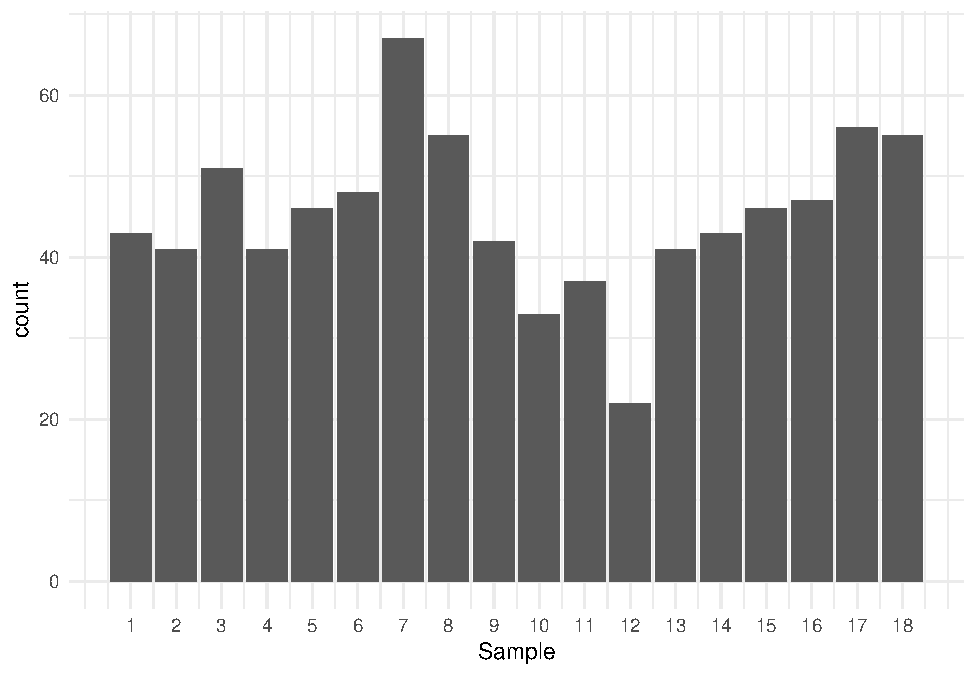
\includegraphics{paper_files/figure-latex/unnamed-chunk-2-1} 

}

\caption{Fossil sampel size for each time period}\label{fig:unnamed-chunk-2}
\end{figure}

\begin{longtable}[]{@{}
  >{\raggedright\arraybackslash}p{(\columnwidth - 4\tabcolsep) * \real{0.3492}}
  >{\raggedright\arraybackslash}p{(\columnwidth - 4\tabcolsep) * \real{0.1905}}
  >{\raggedright\arraybackslash}p{(\columnwidth - 4\tabcolsep) * \real{0.4603}}@{}}
\caption{Traits and trait descriptions. `sc' denotes size correction of
trait against standard length. Names of bones follow Bowne
(\protect\hyperlink{ref-Bowne1994}{1994}) unless otherwise
noted.}\tabularnewline
\toprule()
\begin{minipage}[b]{\linewidth}\raggedright
Trait Name
\end{minipage} & \begin{minipage}[b]{\linewidth}\raggedright
Trait Code
\end{minipage} & \begin{minipage}[b]{\linewidth}\raggedright
Trait Description
\end{minipage} \\
\midrule()
\endfirsthead
\toprule()
\begin{minipage}[b]{\linewidth}\raggedright
Trait Name
\end{minipage} & \begin{minipage}[b]{\linewidth}\raggedright
Trait Code
\end{minipage} & \begin{minipage}[b]{\linewidth}\raggedright
Trait Description
\end{minipage} \\
\midrule()
\endhead
Standard Length & stl & Distance from anterior tip of premaxilla to
posterior end of last vertebra (hypural plate) \\
Dorsal Spine & mds & Number of dorsal spines from 0 to 3 \\
Dorsal Fin Ray & mdf & Number of bones in the dorsal fin posterior to
the third dorsal spine (i.e., soft dorsal fin rays) \\
Anal Fin Ray & maf & Number of bones in the anal fin posterior to the
anal spine (i.e., soft dorsal fin rays) \\
Abdominal Vertebra & mav & Number of vertebrae anterior to the first
vertebra contacting an anal fin pterygiophore (Aguirre et al.~2014) \\
Caudal Vertebra & mcv & Number of vertebrae posterior to and including
the first vertebra contacting an anal fin pterygiophore (Aguirre et
al.~2014) \\
Pterygiophore number & mpt & Number of pterygiophores anterior to but
excluding the pterygiophore under the third dorsal spine, which is
immediately anterior to and contiguous with the dorsal fin \\
Pelvic Spine length & lps.sc & Length from the base of one pelvic spine
above its articulation with the pelvic girdle to its distal tip \\
Ectocoracoid & ect.sc & Length between the anterior and posterior tips
of the shoulder girdle base (i.e., ectocoracoid) \\
Pelvic Girdle & tpg.sc & Length between the anterior to posterior tips
along midline. If vestigial, the sum of longest anterior-posterior axis
for the vestiges \\
Cleithrum length & cle.sc & Length from free dorsal tip to ventral tip
of the cleithrum on the anterior margin of the shoulder girdle (i.e.,
cleithrum) \\
Premaxilla & pmx.sc & Length from the anterior tip of the premaxilla to
the distal tip of the ascending process of the premaxilla \\
Dorsal Spine & Ds\#.sc\# = 1,2,or 3 & Length from the base of a dorsal
spine above the pterygiophore to its distal tip along the anterior
edge \\
Pterygiophore & lpt.sc & Distance between the anterior to posterior tips
of the pterygiophore immediately preceding the 3rd dorsal spine (when
present) \\
\bottomrule()
\end{longtable}

\hypertarget{extant-specimen-data}{%
\subsection{Extant Specimen data}\label{extant-specimen-data}}

To span the gamut of stickleback diversity for our predictive model, we
sampled modern stickleback from lakes containing generalist stickleback
populations (Hendry et al. (\protect\hyperlink{ref-Hendry2009}{2009});
Bolnick (\protect\hyperlink{ref-Bolnick2011}{2011})) and from lakes
containing benthic-limnetic species pairs (Baumgartner et al.~1988;
Schluter and McPhail (\protect\hyperlink{ref-Schluter1992}{1992}))
(Table 2 (What is this?)). The generalist populations were collected by
YES in 2013 and previously described in Stuart et al.
(\protect\hyperlink{ref-Stuart2017}{2017}). These samples were fixed in
formalin, then stained for bone with Alizarin Red in 2013. Benthic and
limnetic specimens were kindly loaned by D. Schluter and his lab at
University of British Columbia. They collected benthic and limnetic
individuals from Enos Lake in 1988 and from Emily Lake, Little Quarry
Lake, Paxton Lake, and Priest Lake in 2018. The Enos specimens had been
fixed whole in formalin and stored in 40\% isopropanol. The specimens
from the other lakes were initially preserved whole in 95\% ethanol in
the field before being gradually transferred to water then formalin in
the lab and ultimately stored in 40\% isopropanol. In 2019, we stained
these specimens for bone using Alizarin Red.

We next replicated fossil data collection (Table 1) on these extant
specimens. Standard length as well as pelvic-spine length on each side
were measured with calipers. We used a dissection microscope to count
dorsal spines, pelvic spines, dorsal-fin rays, and anal-fin rays. Right
and left-side pelvic girdle lengths and ectocoracoid lengths were
measured from ventral photographs taken using a Canon EOS Rebel T7 with
a Tamron 16-300 mm MACRO lens mounted on a leveled Kaiser RS1 copy
stand. Specimens were held in place for ventral photographs using a
small tabletop vise with an attached scale bar. Lateral X-rays were used
to measure dorsal spine length, number of pterygiophores anterior to the
pterygiophore holding the third spine, length of the pterygiophore just
anterior to the third spine, cleithrum length, and pre-maxilla ascending
branch length. We also counted vertebrae from the X-rays: abdominal
vertebrae were counted anterior to the first vertebra with a haemal
spine contacting an anal fin pterygiophore. Caudal vertebrae were
posterior, including the first vertebra with the haemal spine contacting
the anal fin pterygiophore (following Aguirre, Walker, and Gideon
(\protect\hyperlink{ref-Aguirre2014}{2014}). X-rays were taken with an
AXR Hot Shot X-ray Machine (Associated X-ray Corporation) at the Field
Museum of Natural History. Specimens were exposed at 35kV and 4mA. Small
fish were exposed for 7s, medium fish for 8s, and large fish for 10s. We
developed the film and scanned individual images of each fish using the
B\&W Negatives setting on an Epson Perfection 4990 Photo flatbed at 2400
dpi. Measurements from photographs and X-rays were taken with FIJI
(Schindelin et al.~2012) and its plugin ObjectJ
(\url{https://sils.fnwi.uva.nl/bcb/objectj/}). All photographs, X-rays,
and ObjectJ files have been uploaded to Morphosource.org (accession \#
TBD). We dissected individuals from the generalist populations to
determine sex from the gonads. Individuals from the species-pair lakes
were sexed by Schluter and his lab, using a genotyping protocol (confirm
and cite).

The extant data used here consists of a total of 367 specimens all with
known sex. Of these, there are 202 and 165 female and male specimens,
respectively.

\hypertarget{outlier-analysis.}{%
\subsection{Outlier analysis.}\label{outlier-analysis.}}

To check for outliers, we calculated within-group means and standard
deviations for each trait separately for K series fossil specimens
(pooled across samples) and for extant specimens (pooled across lakes).
We noted trait values greater than 3.5 standard deviations from the mean
as potential outliers. We checked whether these potential outliers were
a result of data entry and collection error and corrected them if they
were. We turned the remaining outlier trait values to NAs. (confirm)
(Wait, what? Why? Anything that was 3.5 SD above the mean was recorded
as missing? How do you justify this? )

Missing data imputation, including fossil sex

Quantification and evolution of sexual dimorphism

What covariates do we have in the data: length, what else,

\hypertarget{sec:models}{%
\section{Models}\label{sec:models}}

\hypertarget{imputation-model}{%
\subsection{Imputation Model}\label{imputation-model}}

Let \(\boldsymbol{W}\) be an \((n_{extant} + n_{fossil}) \times 1\)
vector of the covariate gender of the stickleback fish and
\(\boldsymbol{Y}\) be an \((n_{extant} + n_{fossil}) \times K\) matrix
of the \(K\) phenotypes of interest. Because the gender of the
fossilized stickleback fish is unobservable, we further define
\(\boldsymbol{W} = (\boldsymbol{W}_{extant}^T,\boldsymbol{W}_{fossil}^T)^T\)
where \(\boldsymbol{W}_{extant}\) and \(\boldsymbol{W}_{fossil}\) are
the \(n_{extant} \times 1\) and \(n_{fossil} \times 1\) vectors of the
observed extant gender and missing fossil gender, respectively.

We impute the missing gender for the fossil data by sampling from the
posterior predictive distribution
\(P(\boldsymbol{W}_{fossil}|\boldsymbol{W}_{extant},\boldsymbol{Y})\)
using the multiple imputation by chained equations (MICE) algorithm
(Buuren and Groothuis-Oudshoorn (\protect\hyperlink{ref-MICE}{2011}))
with predictive mean matching. Traditionally, the choice for the number
of completed dats sets is a relatively small number such as \(M = 5\) or
\(M = 10\). However, Zhou and Reiter
(\protect\hyperlink{ref-ZhouReiter2009}{2010}) recommend a larger number
of imputed data sets if the data users intend on performing Bayesians
analysis after imputation, which in this case, we do. Therefore, the
imputation algorithm is run to obtain a total of \(M = 100\) completed
datasets. In addition to this, Zhou and Reiter
(\protect\hyperlink{ref-ZhouReiter2009}{2010}) suggests rather than
using Rubin's combining rules to combine across imputed data sets,
instead pool all of the draws from the posterior distributions across
all of the imputed data sets to estimate the posterior distributions of
parameters of interest. We proceed with our Bayesian analysis in this
manner.

\textcolor{red}{Akhil's stuff about validating the imputation model goes here.}

\hypertarget{completed-data-model}{%
\subsection{Completed Data Model}\label{completed-data-model}}

\textcolor{red}{We should note somewhere that we are only using the $W_{fossil}$ in the modeling part.  We drop the $W_{extant}$.  So just note that $W_{ti}$ is really $W_{fossil,ti}$.  Not sure how to say this, but we need to make it clear that we are only using the fossil data for the OU modeling.  Greg, check and see if this makes sense.}

For a given imputed dataset, let \(W_{ij}\) be the imputed gender and
\(\boldsymbol{Y}_{ij}\) be the \(K \times 1\) vector of phenotypes for
stickleback fossil \(j\) at time \(t_i\) where \(i = 1, \ldots, T\) and
\(j = 1,\ldots,n_{t}\). Note, we are inputting only the fossil data into
our model; connecting to the previous section, \(W_{ij}\) and
\(\boldsymbol{Y}_{ij}\) can be interpretted as \(W_{fossil,ij}\) and
\(\boldsymbol{Y}_{fossil,ij}\). In addition, we denote \(Y_{K,ij}\), the
last variable in \(\boldsymbol{Y}_{ij}\), to be the standard length of
the fish, \begin{align}
{Y}_{K,ij} & \overset{iid}{\sim}\left\{\begin{array}{lll} \mathcal{N}(\mu_{K,ft_i},&\sigma_{K}^2), & W_{ij} = \text{Female} \\ \mathcal{N}(\mu_{K,mt_i},&\sigma_{K}^2), & W_{ij} = \text{Male} \end{array}\right..
\label{eq:stl}
\end{align}

It is reasonable to assume that the other continuous traits of
stickleback fish will have some correlation with its standard length
\textbf{(CITATION)}. We account for this by adding an additional
parameter, \(\gamma_k\), into our model. More specifically, if
\(Y_{k,ij}\) is a continuous trait, then \begin{align}
{Y}_{k,ij} & \overset{iid}{\sim}\left\{\begin{array}{llll} \mathcal{N}(\mu_{k,ft_i} + \gamma_kY_{K,ij},\sigma_k^2), & W_{ij} = \text{Female} \\ \mathcal{N}(\mu_{k,mt_i} + \gamma_kY_{K,ij},\sigma_k^2), & W_{ij} = \text{Male} \end{array}\right..
\label{eq:cont}
\end{align}

In addition, we assume that the discrete traits abdominal vertebrae
(mav) and caudal vertebrae (mcv) also have correlation with the standard
length of the fish (\textbf{CITATION}). If \(Y_{k,ij}\) is one of the
above traits, then \begin{align}
{Y}_{k,ij} & \sim \left\{\begin{array}{ll} Poisson(\exp\{\mu_{k,ft_i} + \gamma_kY_{K,ij}\}), & W_{ij} = \text{Female} \\ Poisson(\exp\{\mu_{k,mt_i} + \gamma_kY_{K,ij}\}), & W_{ij} = \text{Male} \end{array}\right..
\label{eq:disc_corr}
\end{align}

For the other discrete traits, we also assume the above model except we
set \(\gamma_k = 0\) because of the assumption of no correlation between
the standard length and these traits. More specifically, we assume
\begin{align}
{Y}_{k,ij} & \sim \left\{\begin{array}{ll} Poisson(\exp\{\mu_{k,ft_i}\}), & W_{ij} = \text{Female} \\ Poisson(\exp\{\mu_{k,mt_i}\}), & W_{ij} = \text{Male} \end{array}\right..
\label{eq:disc_ind}
\end{align}

In the above model descriptions, \(\mu_{k,ft_i}\) and \(\mu_{k,mt_i}\)
model the time-\(t_i\) specific mean of phenotype \(k\) for female and
male stickleback fish, respectively. We point out that, for the discrete
traits, the means are represented by \(\exp\{\mu_{k,ft_i}\}\) and
\(\exp\{\mu_{k,mt_i}\}\) for ease of use in our modeling technique. We
further set \begin{align}
\mu_{k,gt_i} = \beta_{0,kg} + \beta_{1,kg}t_i + u_{k,gt_i},
\label{eq:mu}
\end{align} for \(g \in \{f,m\}\) where \(\beta_{0,kg}\) and
\(\beta_{1,kg}\) are regression parameters of phenotype \(Y_k\) for each
gender, accounting for the possibility of a time-dependent trend in the
mean structure, and \(u_{k,gt_i}\) is the corresponding residual. To
account for potential correlations between the residuals for a given
trait \(k\) and gender \(g\), we fit an Ornstein-Uhlenback (OU) process
(Uhlenbeck and Ornstein (\protect\hyperlink{ref-OUProcess}{1930})). More
specifically, define \(du_{k,gt} = u_{k,g(t + dt)} - u_{k,gt}\), the
change in \(u_k,gt\) for a given trait \(k\) and gender \(g\) over a
miniscule time period \(dt\). The OU process is defined as \begin{align}
du_{k,gt} = -\kappa_k u_{k,gt} dt + \tau_k dW_t,
\label{eq:OU_cont}
\end{align} where \(\kappa_k\) is a parameter associated with the
correlation between \(u_{k,gt}\) and \(u_{k,g(t+dt)}\), \(\tau_k\) is
the standard deviation of the OU process, and \(W_t\) is a standard
Brownian motion. As shown in (Uhlenbeck and Ornstein
(\protect\hyperlink{ref-OUProcess}{1930})), the closed form solution for
the SDE in (\ref{eq:OU_cont}) is \begin{align}
u_{k,gt_i} \overset{iid}{\sim}\mathcal{N}\left(u_{k,gt_{i-1}}\exp\{-\kappa_k(t_{i} - t_{i-1})\} , \frac{\tau_k^2(1 - \exp\{-2\kappa_k(t_{i} - t_{i-1}))\}}{2\kappa_k}\right)
\label{eq:OU_sol}
\end{align} for \(i = 2,\cdots,T\). In a traditional OU process, the
initial value \(u_{k,gt_1}\) is assumed to be a (potentially unknown)
constant, and we discuss the procedure for estimating this value below.

In our empirical study, we analyze the following four nested models for
the mean process outlined in (\ref{eq:mu}):

\begin{itemize}
\item OU with Trend: The mean process for each phenotype $k=1,\cdots,K$ and $g \in \{f,m\}$ as previously defined.
\item OU with No Trend: No linear trend on the mean processes and the overall mean of the phenotype is constant for each gender. This is achieved by setting $\beta_{1,kg} = 0$ in (\ref{eq:mu}) for $k = 1,\cdots,K$ and $g \in \{f,m\}$
\item No OU with Trend: No random fluctuations on the mean processes, i.e. the OU process assumption is not needed. This is achieved by setting $u_{k,gt_i} = 0$ in (\ref{eq:mu}) for $k = 1,\cdots,K$, $g \in \{f,m\}$, and $i = 1,\cdots,T$.
\item No OU with No Trend: The mean for a specific trait and specific gender at each time point is a constant value. This is achieved by setting $\beta_{1,kg} = 0$ and $u_{k,gt_i} = 0$ in (\ref{eq:mu}) for $k = 1,\cdots,K$, $g \in \{f,m\}$, and $i = 1,\cdots,T$.
\end{itemize}

Because we are fitting a dataset with a stochastic structure on the
means of the phenotypes, we analyze the data via a Bayesian analysis.
Bayesian data analysis is also more naturally used when we have to
impute data (\textbf{CITATION}).

Priors: For \(k = 1,\cdots,K\),

\begin{align}
u_{k,gt_1} & \overset{iid}{\sim}\mathcal{N}(0,\tau_{0,k}) \nonumber \\
\sigma_k & \overset{iid}{\sim}\mathcal{N}(0,10)I_{\{\sigma > 0\}} \nonumber \\
\tau_k & \overset{iid}{\sim}\mathcal{N}(0,10)I_{\{\tau > 0\}} \nonumber \\
\tau_{0,k} & \overset{iid}{\sim}\mathcal{N}(0,20)I_{\{\tau > 0\}} \nonumber \\
\kappa_k & \overset{iid}{\sim}\mathcal{N}(0,1)I_{\{\kappa_g > 0\}} \nonumber \\
\gamma_{k} & \overset{iid}{\sim}\mathcal{N}(0,5) \nonumber \\
\beta_{0,kg} & \overset{iid}{\sim}\mathcal{N}(0,100) \nonumber \\
\beta_{1,kg} & \overset{iid}{\sim}\mathcal{N}(0,3) \nonumber \\
\label{eq:priors}
\end{align} We also note that, for the discrete phenotypes in equations
(\ref{eq:disc_corr}) and (\ref{eq:disc_ind}), there is no \(\sigma_k\),
and thus is not sampled for those phenotypes.

All models were built using Team
(\protect\hyperlink{ref-R2022language}{2022}) and (\textbf STAN)

Cornuault (\protect\hyperlink{ref-Cornault2022}{2022}) Bayesian OU
model.

Bayesian Analysis after multiple imputation Zhou and Reiter
(\protect\hyperlink{ref-ZhouReiter2009}{2010}): They recommend using a
large number of imputations. 5 or 10 is too small. We are using M = 100.

\hypertarget{sec:results}{%
\section{Results}\label{sec:results}}

\hypertarget{sec:conclusions}{%
\section{Discsusson, Future work and
conclusions}\label{sec:conclusions}}

We predicted that release from predators would result in niche expansion
and increased sexual dimorphism, based on several studies of modern
stickleback. For example, in lakes where sculpin competitors are absent
and stickleback (Roesti et al.~2023) See Spoljaric and Reimchen 2008,
page 512 right column for references and discussion of differences
between benthic males and limnetic females. Male stickleback are benthic
and littoral (Wootton 1976)\ldots. Reimchen papers in general good for
this section.

\hypertarget{acknowledgements}{%
\section*{Acknowledgements}\label{acknowledgements}}
\addcontentsline{toc}{section}{Acknowledgements}

We thank O. Abughoush, S. Blaine, A. Chaudhary, M. Islam, F. Joaquin, C.
Lawson-Weinert, R. Sullivan, J. Tien, M.P. Travis, and W. Shim for help
with data collection. We thank D. Schluter and S. Blain for loaning
specimens and sharing data. We thank K. Swagel and C. McMahan of the
Field Museum for assistance with specimen x-rays. This research was
supported by NSF grants BSR-8111013, EAR-9870337, and DEB-0322818, the
Center for Field Research (Earthwatch), and the National Geographic
Society (2869-84) to MAB. It was also supported by NSF grants
DEB-1456462 and EAR-2145830 to YES. And NSF DMS-2015374 (GJM)

\hypertarget{supplementary-material}{%
\section*{Supplementary Material}\label{supplementary-material}}
\addcontentsline{toc}{section}{Supplementary Material}

All code for reproducing the analyses in this paper is publicly
available at \url{https://github.com/Akhil-Ghosh/SticklebackProject}

\hypertarget{references}{%
\section*{References}\label{references}}
\addcontentsline{toc}{section}{References}

\hypertarget{refs}{}
\begin{CSLReferences}{1}{0}
\leavevmode\vadjust pre{\hypertarget{ref-Aguirre2014}{}}%
Aguirre, Windsor E, Kendal Walker, and Shawn Gideon. 2014. {``Tinkering
with the Axial Skeleton: Vertebral Number Variation in Ecologically
Divergent Threespine Stickleback Populations.''} \emph{Biol. J. Linn.
Soc. Lond.} 113 (1): 204--19.

\leavevmode\vadjust pre{\hypertarget{ref-Bell2009}{}}%
Bell, M A. 2009. {``Implications of a Fossil Stickleback Assemblage for
Darwinian Gradualism.''} \emph{J. Fish Biol.} 75 (8): 1977--99.

\leavevmode\vadjust pre{\hypertarget{ref-Bell2006}{}}%
Bell, Michael A, Matthew P Travis, and D Max Blouw. 2006. {``Inferring
Natural Selection in a Fossil Threespine Stickleback.''}
\emph{Paleobiology} 32 (4): 562--77.

\leavevmode\vadjust pre{\hypertarget{ref-BellEtAl1993}{}}%
Bell, Orti, M. A., and J. P. Koenings. 1993. {``Evolution of Pelvic
Reduction in Threespine Sticklebacks: A Test of Competing Hypotheses.''}
\emph{Evolution} 47: 906--14.

\leavevmode\vadjust pre{\hypertarget{ref-Blain2022}{}}%
Blain, S A. 2022. \emph{Evolutionary Outcomes of Interactions Among
Phenotypes in Post-Glacial Lakes}. University of British Columbia,
Canada.

\leavevmode\vadjust pre{\hypertarget{ref-Bolnick2011}{}}%
Bolnick, Daniel I. 2011. {``Sympatric Speciation in Threespine
Stickleback: Why Not?''} \emph{Int. J. Ecol.} 2011: 1--15.

\leavevmode\vadjust pre{\hypertarget{ref-Bolnick2003}{}}%
Bolnick, Daniel I, and Michael Doebeli. 2003. {``Sexual Dimorphism and
Adaptive Speciation: Two Sides of the Same Ecological Coin.''}
\emph{Evolution} 57 (11): 2433--49.

\leavevmode\vadjust pre{\hypertarget{ref-Bolnick2010}{}}%
Bolnick, Daniel I, Travis Ingram, William E Stutz, Lisa K Snowberg, On
Lee Lau, and Jeff S Paull. 2010. {``Ecological Release from
Interspecific Competition Leads to Decoupled Changes in Population and
Individual Niche Width.''} \emph{Proc. Biol. Sci.} 277 (1689): 1789--97.

\leavevmode\vadjust pre{\hypertarget{ref-Bolnick2008}{}}%
Bolnick, Daniel I, and On Lee Lau. 2008. {``Predictable Patterns of
Disruptive Selection in Stickleback in Postglacial Lakes.''} \emph{Am.
Nat.} 172 (1): 1--11.

\leavevmode\vadjust pre{\hypertarget{ref-Bowne1994}{}}%
Bowne, P S. 1994. {``Systematics and Morphology of the
Gasterosteiformes.''} In \emph{The Evolutionary Biology of the
Threespine Stickleback}, edited by M A Bell and S A Foster. Oxford, UK:
Oxford University Press.

\leavevmode\vadjust pre{\hypertarget{ref-Butler2007}{}}%
Butler, Marguerite A, Stanley A Sawyer, and Jonathan B Losos. 2007.
{``Sexual Dimorphism and Adaptive Radiation in Anolis Lizards.''}
\emph{Nature} 447 (7141): 202--5.

\leavevmode\vadjust pre{\hypertarget{ref-MICE}{}}%
Buuren, Stef van, and Karin Groothuis-Oudshoorn. 2011. {``Mice:
Multivariate Imputation by Chained Equations in r.''} \emph{Journal of
Statistical Software} 45 (3): 1--67.
\url{https://doi.org/10.18637/jss.v045.i03}.

\leavevmode\vadjust pre{\hypertarget{ref-Cooper2011}{}}%
Cooper, Idelle A, R Tucker Gilman, and Janette Wenrick Boughman. 2011.
{``Sexual Dimorphism and Speciation on Two Ecological Coins: Patterns
from Nature and Theoretical Predictions.''} \emph{Evolution} 65 (9):
2553--71.

\leavevmode\vadjust pre{\hypertarget{ref-Cornault2022}{}}%
Cornuault, Josselin. 2022. {``Bayesian Analyses of Comparative Data with
the Ornstein--Uhlenbeck Model: Potential Pitfalls.''} \emph{Systematic
Biology} 71 (6): 1524--40. \url{https://doi.org/10.1093/sysbio/syac036}.

\leavevmode\vadjust pre{\hypertarget{ref-deLisleNco2018}{}}%
De Lisle, S. Paiva, S. P., and L. Rowe. 2018. {``Habitat Partitioning
During Character Displacement Between the Sexes.''} \emph{Biology
Letters} 14: 20180124.

\leavevmode\vadjust pre{\hypertarget{ref-deLisleRowe2015}{}}%
De Lisle, S. P., and L. Rowe. 2015. {``Ecological Character Displacement
Between the Sexes.''} \emph{The American Naturalist} 186: 693--707.

\leavevmode\vadjust pre{\hypertarget{ref-Hendry2009}{}}%
Hendry, A P, D I Bolnick, D Berner, and C L Peichel. 2009. {``Along the
Speciation Continuum in Sticklebacks.''} \emph{J. Fish Biol.} 75 (8):
2000--2036.

\leavevmode\vadjust pre{\hypertarget{ref-Herrmann2021}{}}%
Herrmann, Nicholas C, James T Stroud, and Jonathan B Losos. 2021. {``The
Evolution of 'Ecological Release' into the 21st Century.''} \emph{Trends
Ecol. Evol.} 36 (3): 206--15.

\leavevmode\vadjust pre{\hypertarget{ref-Hone2017}{}}%
Hone, David W E, and Jordan C Mallon. 2017. {``Protracted Growth Impedes
the Detection of Sexual Dimorphism in Non-Avian Dinosaurs.''}
\emph{Palaeontology} 60 (4): 535--45.

\leavevmode\vadjust pre{\hypertarget{ref-Hunt2008}{}}%
Hunt, Gene, Michael A Bell, and Matthew P Travis. 2008. {``Evolution
Toward a New Adaptive Optimum: Phenotypic Evolution in a Fossil
Stickleback Lineage.''} \emph{Evolution} 62 (3): 700--710.

\leavevmode\vadjust pre{\hypertarget{ref-little2002statistical}{}}%
Little, R. J. A., and D. B. Rubin. 2002. \emph{Statistical Analysis with
Missing Data}. Wiley Series in Probability and Mathematical Statistics.
Probability and Mathematical Statistics. Wiley.
\url{http://books.google.com/books?id=aYPwAAAAMAAJ}.

\leavevmode\vadjust pre{\hypertarget{ref-Reimchen2016}{}}%
Reimchen, D. Steeves, T. E. 2016. {``Sex Matters for Defence and Trophic
Traits of Threespine Stickleback.''} \emph{Evolutionary Ecology
Research} 17: 459-485-.

\leavevmode\vadjust pre{\hypertarget{ref-Reimchen1980}{}}%
Reimchen, T. E. 1980. {``Spine Deficiency and Polymorphism in a
Poulation of Gasterosteus Aculeatus: An Adaptation to Predators?''}
\emph{Canadian Journal of Zoology} 58: 1232--44.

\leavevmode\vadjust pre{\hypertarget{ref-Reimchen1994}{}}%
---------. 1994. {``Predators and Morphological Evolution in Threespine
Stickleback.''} In \emph{The Evolutionary Biology of the Threespine
Stickleback}, edited by M A Bell and S A Foster. Oxford, UK: Oxford
University Press.

\leavevmode\vadjust pre{\hypertarget{ref-ReimchenNosil2004}{}}%
Reimchen, T. E., and P. Nosil. 2004. {``Variable Predation Regimes
Predict the Evolution of Sexual Dimorphism in a Population of Threespine
Stickleback.''} \emph{Evolution} 58 (6): 1274--81.

\leavevmode\vadjust pre{\hypertarget{ref-Roestietal2023}{}}%
Roesti, J. S. Groh, M, and D. Schluter. 2023. {``Species Divergence
Under Competition and Shared Predation.''} \emph{Ecology Letters} 26:
111--23.

\leavevmode\vadjust pre{\hypertarget{ref-SaittaEtAl2020}{}}%
Saitta, Evan T, Maximilian T Stockdale, Nicholas R Longrich, Vincent
Bonhomme, Michael J Benton, Innes C Cuthill, and Peter J Makovicky.
2020. {``An Effect Size Statistical Framework for Investigating Sexual
Dimorphism in Non-Avian Dinosaurs and Other Extinct Taxa.''}
\emph{Biological Journal of the Linnean Society} 131 (2): 231--73.
\url{https://doi.org/10.1093/biolinnean/blaa105}.

\leavevmode\vadjust pre{\hypertarget{ref-Schluter1992}{}}%
Schluter, D, and J D McPhail. 1992. {``Ecological Character Displacement
and Speciation in Sticklebacks.''} \emph{Am. Nat.} 140 (1): 85--108.

\leavevmode\vadjust pre{\hypertarget{ref-Shine1989}{}}%
Shine, R. 1989. {``Ecological Causes for the Evolution of Sexual
Dimorphism: A Review of the Evidence.''} \emph{Q. Rev. Biol.} 64 (4):
419--61.

\leavevmode\vadjust pre{\hypertarget{ref-SpoljaricReimchen2008}{}}%
Spoljaric, M. A., and T. E. Reimchen. 2008. {``Habitat-Dependent
Reduction of Sexual Dimorphism in Geometric Body Shape of Haida Gwaii
Threespine Stickleback.''} \emph{Biological Journal of the Linnean
Society} 95: 505--16.

\leavevmode\vadjust pre{\hypertarget{ref-Stuart2021}{}}%
Stuart, Yoel E, J William Sherwin, Ambika Kamath, and Thor Veen. 2021.
{``Male and Female Anolis Carolinensis Maintain Their Dimorphism Despite
the Presence of Novel Interspecific Competition.''} \emph{Evolution} 75
(11): 2708--16.

\leavevmode\vadjust pre{\hypertarget{ref-Stuart2020}{}}%
Stuart, Yoel E, Matthew P Travis, and Michael A Bell. 2020. {``Inferred
Genetic Architecture Underlying Evolution in a Fossil Stickleback
Lineage.''} \emph{Nat. Ecol. Evol.} 4 (11): 1549--57.

\leavevmode\vadjust pre{\hypertarget{ref-Stuart2017}{}}%
Stuart, Yoel E, Thor Veen, Jesse N Weber, Dieta Hanson, Mark Ravinet,
Brian K Lohman, Cole J Thompson, et al. 2017. {``Contrasting Effects of
Environment and Genetics Generate a Continuum of Parallel Evolution.''}
\emph{Nat. Ecol. Evol.} 1 (6): 158.

\leavevmode\vadjust pre{\hypertarget{ref-R2022language}{}}%
Team, R Core. 2022. \emph{R: A Language and Environment for Statistical
Computing}. Vienna, Austria: R Foundation for Statistical Computing.
\url{https://www.R-project.org/}.

\leavevmode\vadjust pre{\hypertarget{ref-OUProcess}{}}%
Uhlenbeck, G. E., and L. S. Ornstein. 1930. {``On the Theory of the
Brownian Motion.''} \emph{Phys. Rev.} 36 (September): 823--41.
\url{https://doi.org/10.1103/PhysRev.36.823}.

\leavevmode\vadjust pre{\hypertarget{ref-Voje2022}{}}%
Voje, Kjetil L, Michael A Bell, and Yoel E Stuart. 2022. {``Evolution of
Static Allometry and Constraint on Evolutionary Allometry in a Fossil
Stickleback.''} \emph{J. Evol. Biol.} 35 (3): 423--38.

\leavevmode\vadjust pre{\hypertarget{ref-Schoener1968}{}}%
W., Schoener T. 1968. {``The Anolis Lizards of Bimini: Resource
Partitioning in a Complex Fauna.''} \emph{Ecology} 49: 704--26.

\leavevmode\vadjust pre{\hypertarget{ref-ZhouReiter2009}{}}%
Zhou, X., and J. Reiter. 2010. {``A Note on Bayesian Inference After
Multiple Imputation.''} \emph{The American Statistician} 64 (2):
159--63.

\end{CSLReferences}

\end{document}
